\documentclass[runningheads]{llncs}
\usepackage{graphicx}
\usepackage{amsmath,amssymb} % define this before the line numbering.
\usepackage{ruler}
\usepackage{color}
\usepackage{subfig}
\usepackage[width=122mm,left=12mm,paperwidth=146mm,height=193mm,top=12mm,paperheight=217mm]{geometry}
\usepackage[pagebackref=true,breaklinks=true,colorlinks,bookmarks=false]{hyperref}
\begin{document}
% \renewcommand\thelinenumber{\color[rgb]{0.2,0.5,0.8}\normalfont\sffamily\scriptsize\arabic{linenumber}\color[rgb]{0,0,0}}
% \renewcommand\makeLineNumber {\hss\thelinenumber\ \hspace{6mm} \rlap{\hskip\textwidth\ \hspace{6.5mm}\thelinenumber}}
% \linenumbers
\pagestyle{headings}

% Definitions
\newcommand{\argmax}{\operatornamewithlimits{argmax}}
\def\subsectionautorefname{section}
\definecolor{light-gray}{gray}{0.5}
\newcommand{\aside}[1]{\textcolor{light-gray}{\emph{#1}}}
\newcommand{\todo}[1]{\textcolor{red}{\emph{#1}}}
\newcommand{\cut}[1]{\textcolor{light-gray}{#1}}
\newcommand{\comment}[1]{}

\mainmatter
\def\ECCV12SubNumber{1617}  % Insert your submission number here

\title{Timely Object Recognition}

\titlerunning{ECCV-12 submission ID \ECCV12SubNumber}

\authorrunning{ECCV-12 submission ID \ECCV12SubNumber}

\author{Anonymous ECCV submission}
\institute{Paper ID \ECCV12SubNumber}

\maketitle

\begin{abstract}
In a large visual multi-class detection system, the problem of timeliness of results is crucial.
We are motivated by situations where running all detectors would take an unacceptably long time, and that the best answer must be given by some deadline.
Our system for multi-class detection aims to give the best possible results at any single point after a start time; it is terminated at a deadline time.
Toward this goal, we formulate a dynamic policy, guided by inference of the contents of the image, to decide which detector to deploy next.
We evaluate parametrizations of the policy with respect to performance in the novel AP vs. Time evaluation on the PASCAL VOC dataset.
\end{abstract}

\section{Introduction}

In recent years, the computer vision field has converged on a general method for object detection, and a standard evaluation of results.
Most current state-of-the-art object detection systems consist of three tasks: proposing regions of the image, evaluating a given region for presence of an object of a given category, and post-processing the results.
In the evaluation ground truth, each object is most commonly assumed to belong to one of a fixed set of classes; its location is approximated by placing a bounding box around pixels belonging to it.
Large datasets of such human annotations are used for evaluation of detection algorithms~\cite{pascal-voc-2010,imagenet_cvpr09}.

With few exceptions, current detection systems are not inherently multi-class.
Instead, separate detectors are trained per class, and they are deployed and evaluated independently.
The evaluation of multi-class performance, if at all given, consists of averaging the per-class metrics.
Some notable papers do make multi-class detection a priority, and accordingly evaluate in a multi-class setting, where false positives can be generated both by incorrect localization and incorrect labeling.
State-of-the-art detection systems also do not generally make efficiency a goal.

\begin{figure}[ht!]
\center{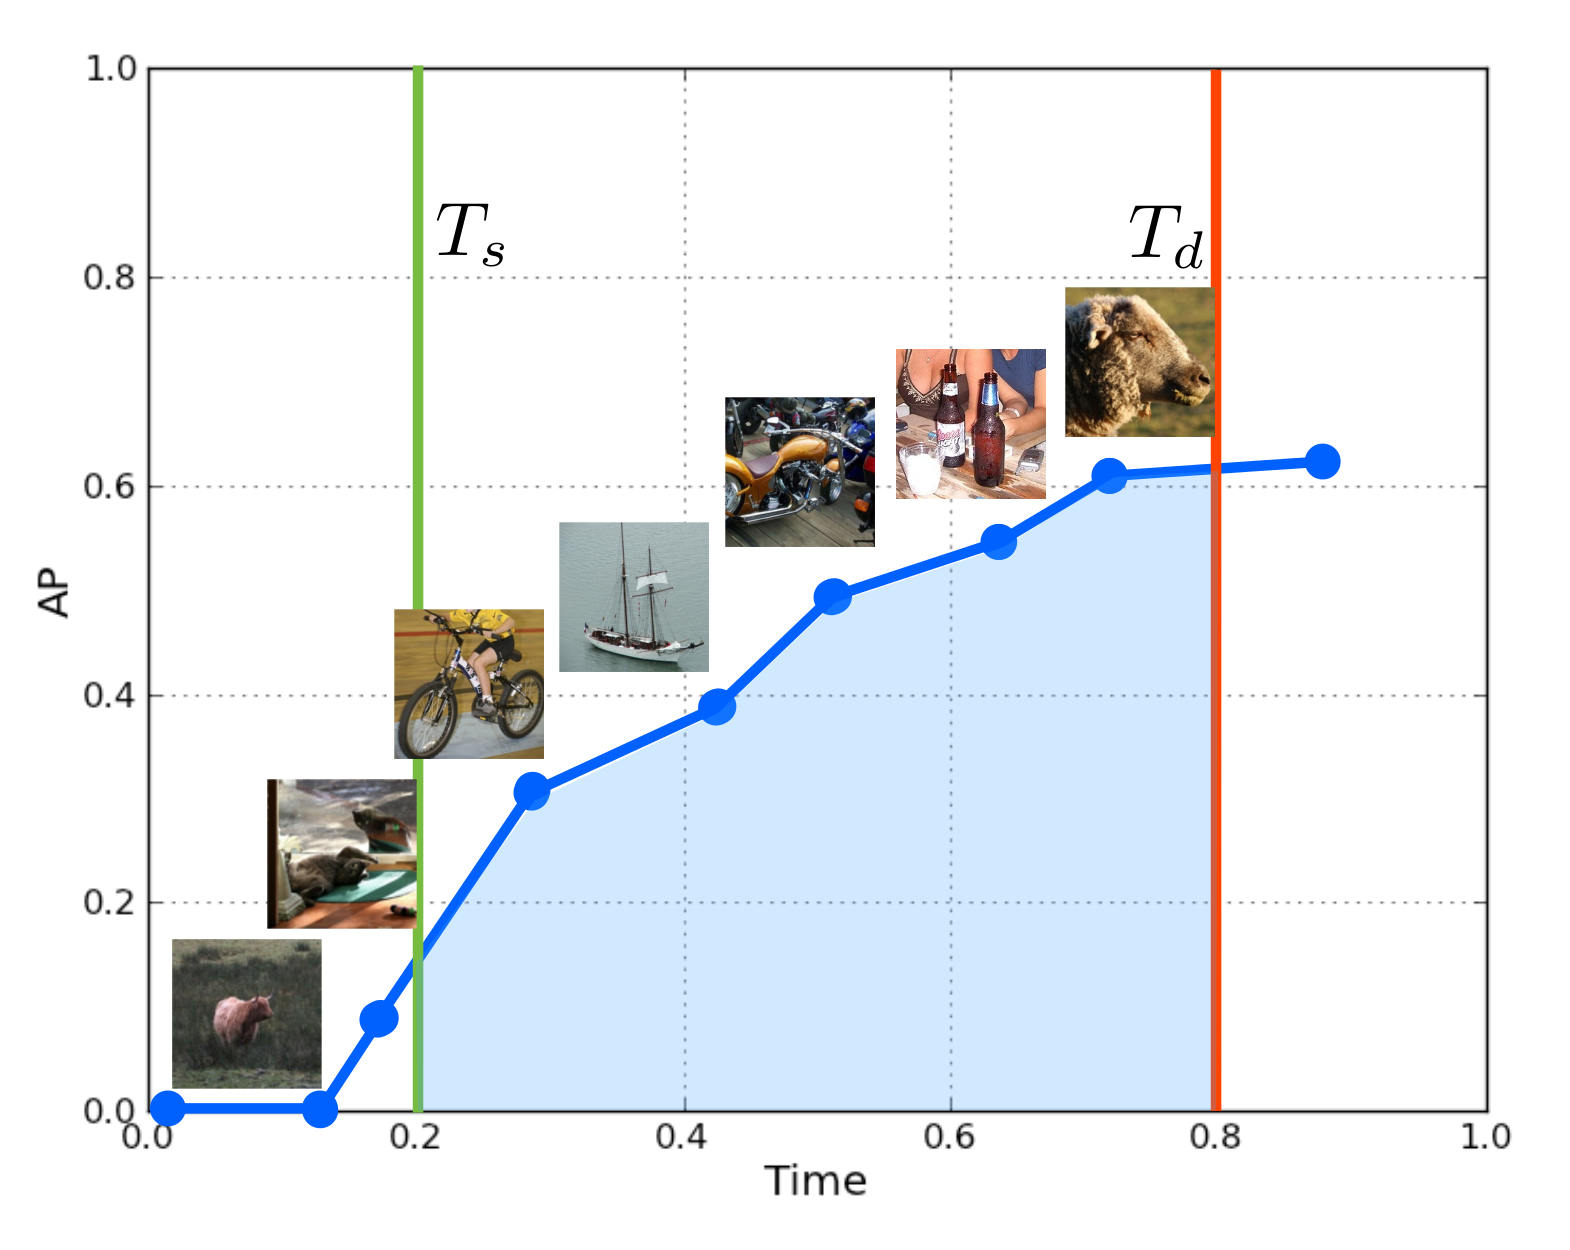
\includegraphics[width=0.56\linewidth]
    {figures/evaluation_thumbs.png}}
  \caption{We aim for \emph{Anytime} performance within the bounds of the curve. That is, the policy should give the best possible answer at any time from start time $T_s$ to deadline $T_d$.}
  \label{fig:evaluation}
\end{figure}

It is of course important to refrain from locking object recognition research into a single detector architecture with a focus only on increasing efficiency.
That said, there are applications for which performance truly is time-sensitive.
In robotics, a small finite amount of processing power per unit time is all that is available for robust object detection if the robot is to usefully interact with humans.
In large-scale detection system deployments, such as for image search, results need to be obtained quickly per image as the number of images to process is large and growing.
When processing large photo collection on end-user machines for immediate consumer navigation, the same is true.

In all these cases, an acceptable answer at a reasonable time may be more valuable than the best answer given too late.
Furthermore, the value of the answer depends largely on the target application.

A hypothetical recognition system for a vision-based advertising deployment presents a case study.
The system will have different accuracies for objects of different classes; detections will have different values based on confidence and class; and the queue of unprocessed images will vary in size.
The most rational detection strategy in such an environment should depend on all of these variables.

We argue that the key to tackling such problems of dynamic recognition resource allocation is to start asking a new question:
\emph{What is the best performance we can get on a budget?}
To answer it, we consider the evaluation metric of performance vs. time, presented in Figure~\ref{fig:evaluation} and discussed further in the text.

Our goal is a dynamic policy for selecting classifiers or detectors to achieve the highest recognition performance under this evaluation.
 % includes Evaluation section

\section{Multi-class Recognition Policy} \label{sec:tech}

Our goal is a multi-class recognition policy $\pi$ that takes an image $\mathcal{I}$ and outputs a list of multi-class detection results by running detector and other \emph{actions} sequentially.

The policy repeatedly selects an action $a_i \in \mathcal{A}$, executes it, receiving observations $o_i$, and then selects the next action.
The set of actions $\mathcal{A}$ can include both classifiers and detectors: anything that would be useful for inferring the contents of the image.

Each action $a_i$ has an expected cost $c(a_i)$ of execution.
Depending on the setting, the cost can be defined in terms of algorithmic runtime analysis, an idealized property such as number of \emph{flops}, or simply the empirical runtime on specific hardware.
We take the empirical approach: every executed action advances $t$, the \emph{time into episode}, by its empirical runtime.

As shown in Figure~\ref{fig:figure1}, the system is given two times: the setup time $T_s$ and deadline $T_d$.
From the setup time to the deadline, we want to obtain the best possible answer if stopped at any given time.
A single-number metric that corresponds to this objective is the area captured under the curve between the start and deadline bounds, normalized by the total area possible.
We evaluate policies by this more robust metric and not simply by the final performance at deadline time for the same reason that Average Precision is used instead of a fixed Precision vs. Recall point in the conventional evaluations.

\subsection{Sequential Execution}
An \emph{open-loop} policy takes actions in a sequence that does not depend on observations received from previous actions.
The common classifier cascade is an example \cite{Viola2001}.
In contrast, our goal is to learn a dynamic, or \emph{closed-loop}, policy, which would exploit the signal in scene and inter-object context for a maximally efficient path through the actions.

We refer to the basis for the decisions made by the decision process as the \emph{state} $s$.
The state includes the currently believed distribution over class presence variables $P(\mathbf{C}) = P(C_1, \dots, C_K)$, where we write $P(C_k)$ to mean $P(C_k=1)$

Additionally, the state records the fact that an action $a_i$ has been taken by adding it to the initially empty set $\mathcal{O}$ and recording the resulting observations $o_i$.
We refer to the current set of observations as $\mathbf{o} = \{o_i | a_i \in \mathcal{O}\}$.
The state also keeps track of the time into episode $t$, and the setup and deadline times $T_s,T_d$.

A recognition \emph{episode} takes an image $\mathcal{I}$ and proceeds from the initial state $s^0$ and action $a^0$ to the next pair $(s^1,a^1)$, and so on until $(s^J,a^J)$, where $J$ is the last step of the process with $t \le T_d$.
At that point, the policy is terminated, and a new episode can begin on a new image.

The specific actions we consider in the following exposition are detector actions $a_{{det}_i}$, where ${det}_i$ is a detector class $C_i$, and a scene-level context action $a_{gist}$, which updates the probabilities of all classes.

\subsection{Selecting actions} \label{sec:value}
As our goal is to pick actions dynamically, we want a function $Q(s,a): S \times \mathcal{A} \mapsto \mathbb{R}$, where $S$ is the space of all possible states, to assign a value to a potential action, given the current state of the decision process.
We can then define the desired policy $\pi$ as simply taking the (untaken) action with the maximum value:
\begin{align}
\pi(s) = \argmax_{a_i \in \mathcal{A} \setminus \mathcal{O}} Q(s,a_i)
\end{align}

Although the action space $\mathcal{A}$ is quite manageable, consisting of the detectors and classifier we would like to run on the image, the space of possible states $S$ is infinite.
Therefore we cannot learn a tabular representation of $Q(s,a)$, and must use function approximation to represent it \cite{Sutton1998}.
We featurize the state-action pair and assume linear structure: $Q^\pi(s,a_i) = \theta_\pi^\top  \phi(s,a_i)$.

The policy's performance at time $t$ is determined by the detections that are part of the set of observations $\mathbf{o}^j$ at the last state $s^j$ before $t$.
Therefore, the final AP vs. Time evaluation of an episode is a function of the history of execution $h=s^0,s^1,\dots,s^J$.

We refer to the final evaluation function as $eval(h,T_s,T_d)$, and it is precisely the area under the AP vs. Time curve between $T_s$ and $T_d$ (normalized by total possible area), as determined by the detections in $\mathbf{o}^j$ for all steps $j$ in the episode.

As shown in \autoref{fig:rewards}, this evaluation function is additive per action, as each action can generate detections that either raise or lower the AP of all detections so far ($\Delta ap$) and takes a certain time ($\Delta t$).
From these and $T_s$ and $T_d$, we can find the area under the curve that was contributed by the action.

Specifically, as shown in Figure~\ref{fig:rewards}, we define the \emph{reward} of an action as
\begin{align}\label{eq:advanced}
R(s^j,a_i) = \Delta \text{ap}_i (t_T^j-\frac{1}{2}\Delta t_i)
\end{align}
where $t_T^j$ and $\text{ap}^j$ are the time left until deadline and the AP at state $s^j$, and $\Delta t_i$ and $\Delta \text{ap}_i$ are the time taken and AP change produced by the action $a_i$.
(For clarity of exposition, we do not account for $T_s$ here.)

We can then represent the final evaluation $eval(h,T_s,T_d)$ in terms of individual rewards: $\sum_{j=0}^J R(s^j,a^j)$.

And we can represent the expected value of the final evaluation recursively in terms of the value function:
\begin{align} \label{eq:recursive_value}
Q^\pi(s^j,a_i) = \mathbb{E}_{s^{j+1}} [R(s^j,a_i) + \gamma Q\pi(s^{j+1},\pi(s^{j+1}))]
\end{align}
where $\gamma \in [0,1]$ is a \emph{discount} value that can mitigate the effects of increasing state-transition uncertainty over long episodes.

\subsection{Learning the policy}
While we can't directly compute the expectation in \eqref{eq:recursive_value}, we can sample it by running actual episodes to gather $<s,a,r,s'>$ samples, where $r$ is the reward obtained by taking action $a$ in state $s$, and $s'$ is the following state.

Learning the policy is then a problem of repeatedly gathering samples with the current policy, minimizing the error between the discounted reward to the end of the episode as predicted by our current $Q(s^j,a_i)$ and the actual values gathered, and updating the policy with the resulting weights.
This is fitted Q-iteration, a variant of generalized policy iteration \cite{Ernst2005,Sutton1998}.

We use $L_2$-regularized regression to minimize the error.
We run $15$ iterations of accumulating samples by running $350$ episodes, starting with a baseline policy which will be described in \autoref{sec:evaluation}, and cross-validating the regularization parameter at each iteration; samples are not thrown away between iterations.

A meta-parameter of the approach is the discount $\gamma$.
With $\gamma=0$, the value function is determined entirely by the immediate reward.
Learning in this case can only result in completely greedy policies.

With $\gamma=1$, the value function is determined by the expected rewards to the end of the episode, and so should be a close approximation to the final evaluation metric.
However, the highest value for $\gamma$ is not necessarily best if the action-value function is not expressive enough to represent the actual state transition behavior of the world.
We experiment with several values of $\gamma$, and find a mid-level value ($0.4$) to work best.

\subsection{Feature representation}
Our policy is at its base determined by a linear function of the features of the state: $\pi(s) = \argmax_{a_i \in \mathcal{A} \setminus \mathcal{O}} \theta_\pi^\top \phi(s,a_i)$.
Since we want to be able to learn a dynamic policy, the observations $\mathbf{o}$ that are part of the state $s$ should play a role in determining the value of a potential action.

We include the following quantities as features $\phi(s,a)$:
\begin{description}
\item[$P(C_a)$] The prior probability of the class that corresponds to the detector of action $a$
\item[$P(C_0|\mathbf{o}) \ldots P(C_K|\mathbf{o})$] The probabilities of all classes, conditioned on the current set of observations.
\item[$H(C_0|\mathbf{o}) \ldots H(C_K|\mathbf{o})$] The entropies of all classes, conditioned on the current set of observations.
\end{description}

Additionally, we include the mean and maximum entropies of all classes, the expected time (cost) of the action, and time features that represent the times until start and deadline, for a total of $F$ features.

We note that this setup is commonly used to solve Markov Decision Processes \cite{Sutton1998}.
There are two related limitations of MDPs when it comes to most systems of interesting complexity, however: the state has to be functionally approximated instead of exhaustively enumerated; and some aspects of the state are not observed, making the problem a Partially Observed MDP (POMDP), for which exact solution methods are intractable for all but rather small problems \cite{Roy2002}.

There isn't much to do about the necessity of approximating the state but design good features.
Our initial solution to the partial observability problem is to include uncertainty features into the feature representation to \emph{augment} the MDP \cite{Kwok2004}.

To formulate learning the policy as a single regression problem, we represent the features in block form, where $\phi(s,a_i)$ is a vector of size $F|\mathcal{A}|$, with all values set to $0$ except for the block corresponding to $a_i$.

As an illustration, we visualize the learned weights on these features in \autoref{fig:weights}, reshaped such that each row shows the weights learned for an action, in order.
The featurization for the $a_{gist}$ scene-context action, which concerns all classes, omits the first $P(C_a)$ feature.

\begin{figure}[h!]
\centering
\subfloat[Greedy]{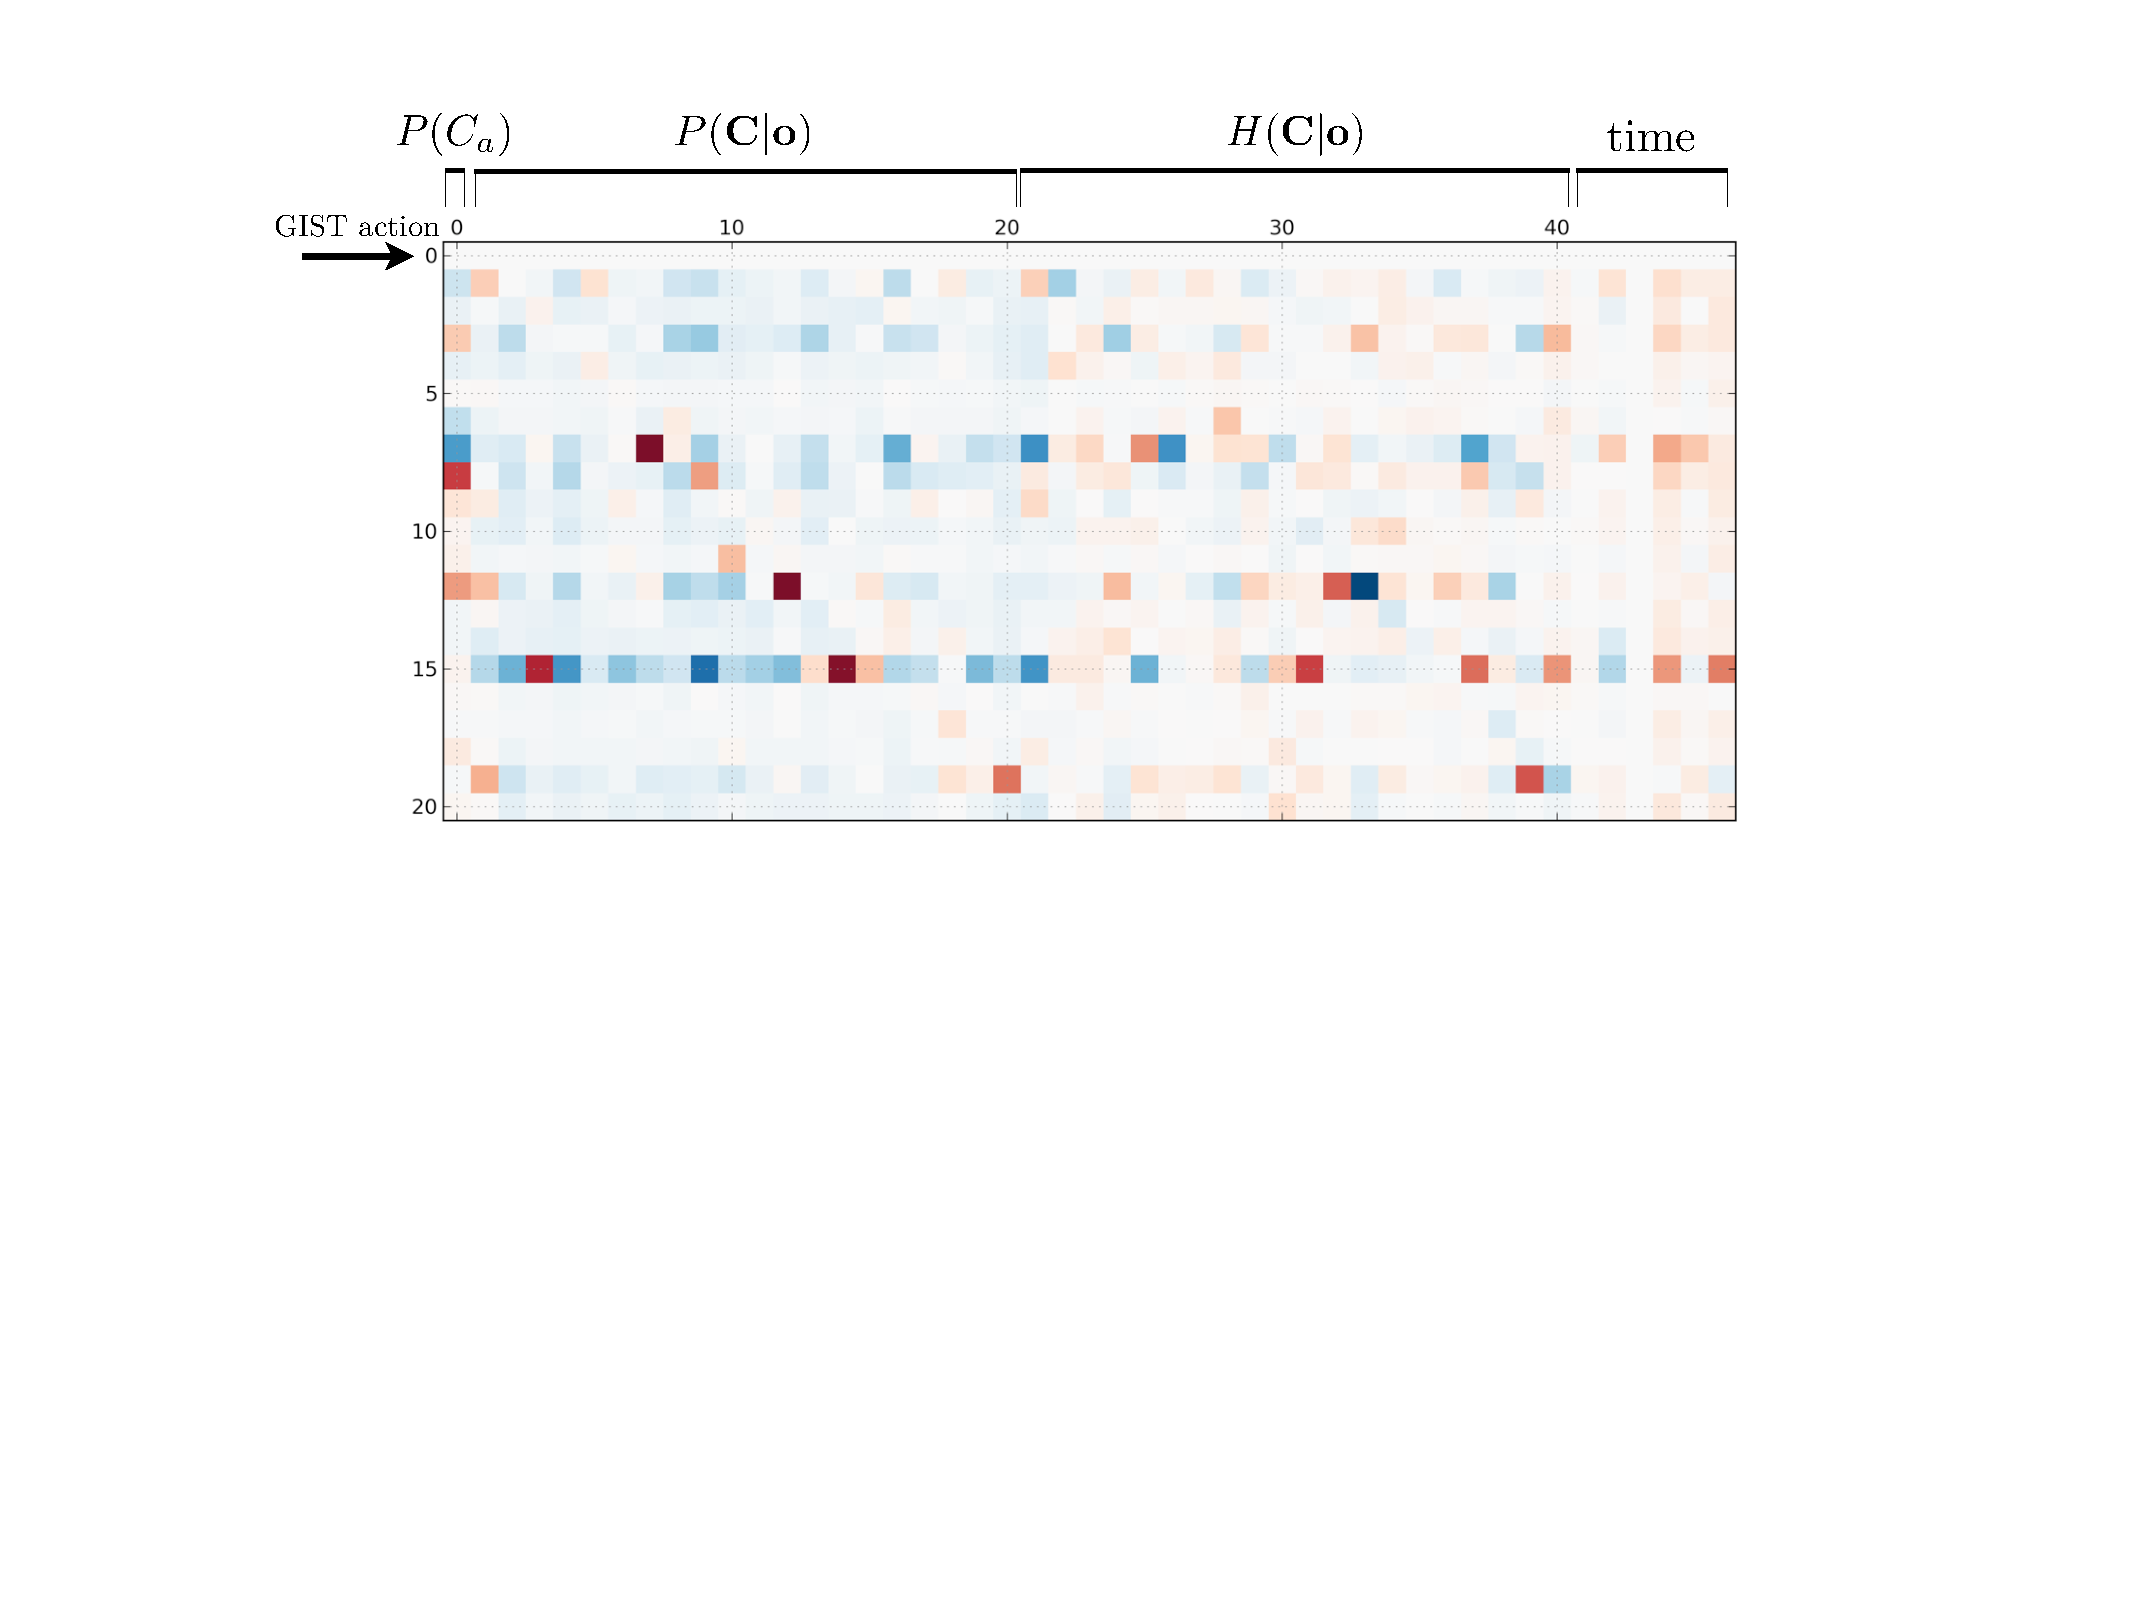
\includegraphics[width=0.49\linewidth]{../figures/weights_greedy}}
\subfloat[RL]{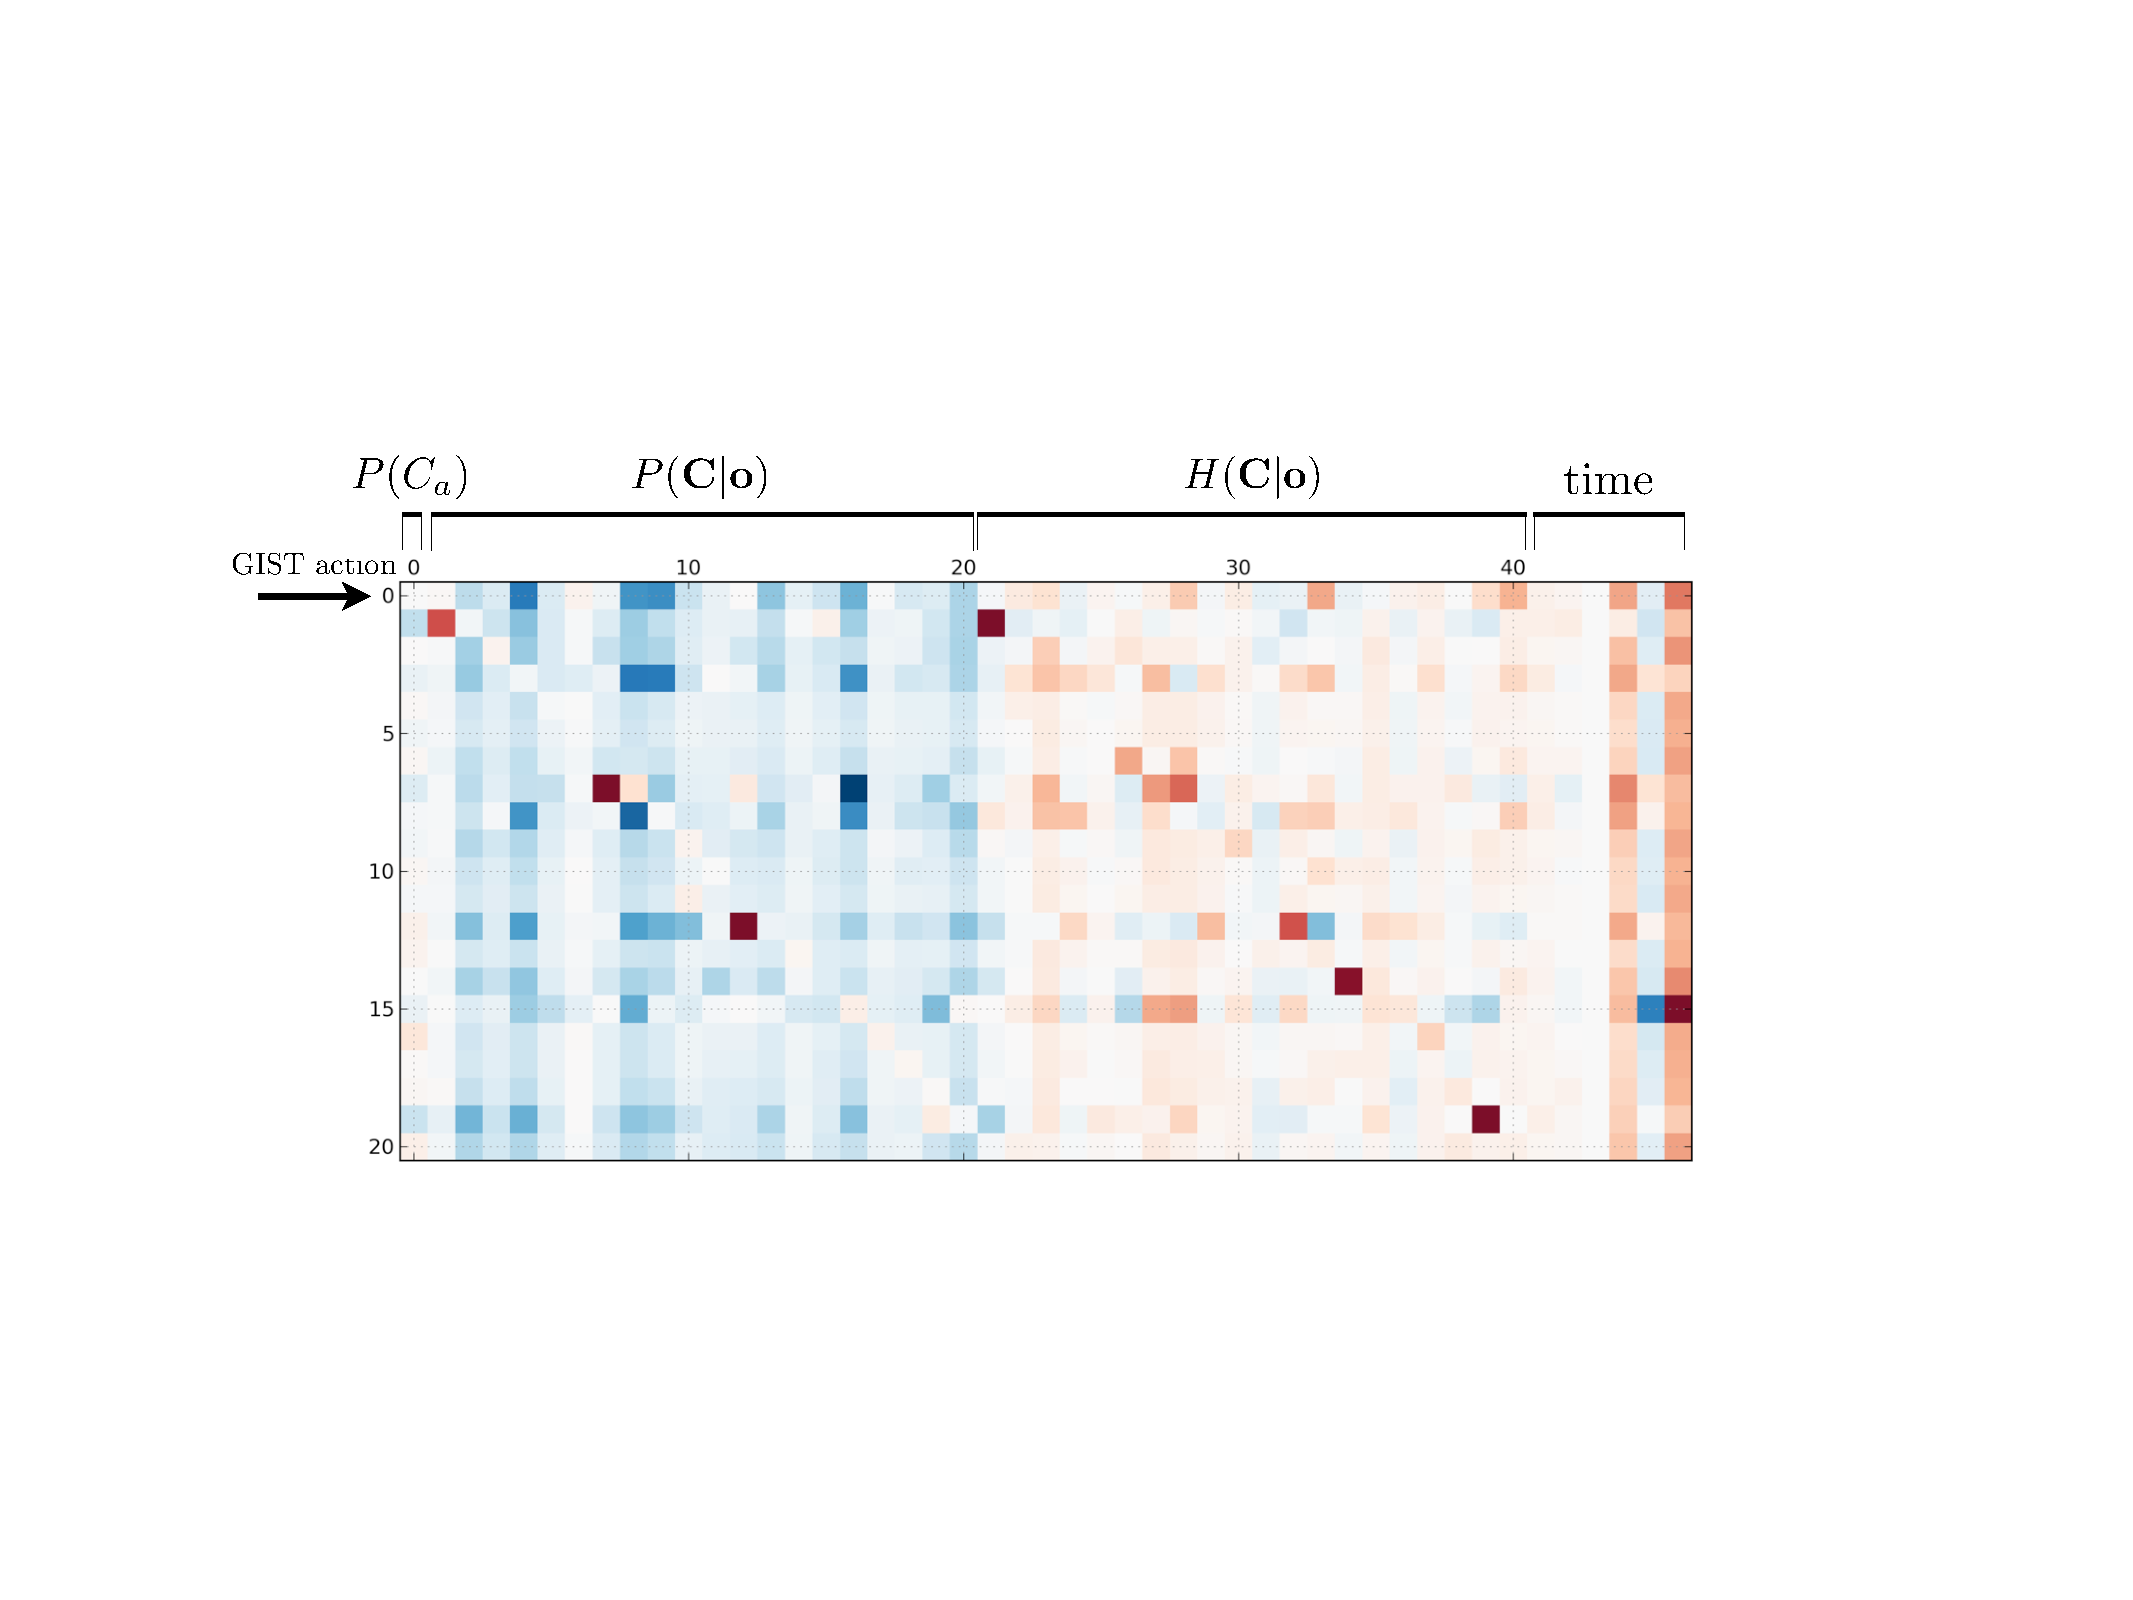
\includegraphics[width=0.49\linewidth]{../figures/weights_rl}}
% 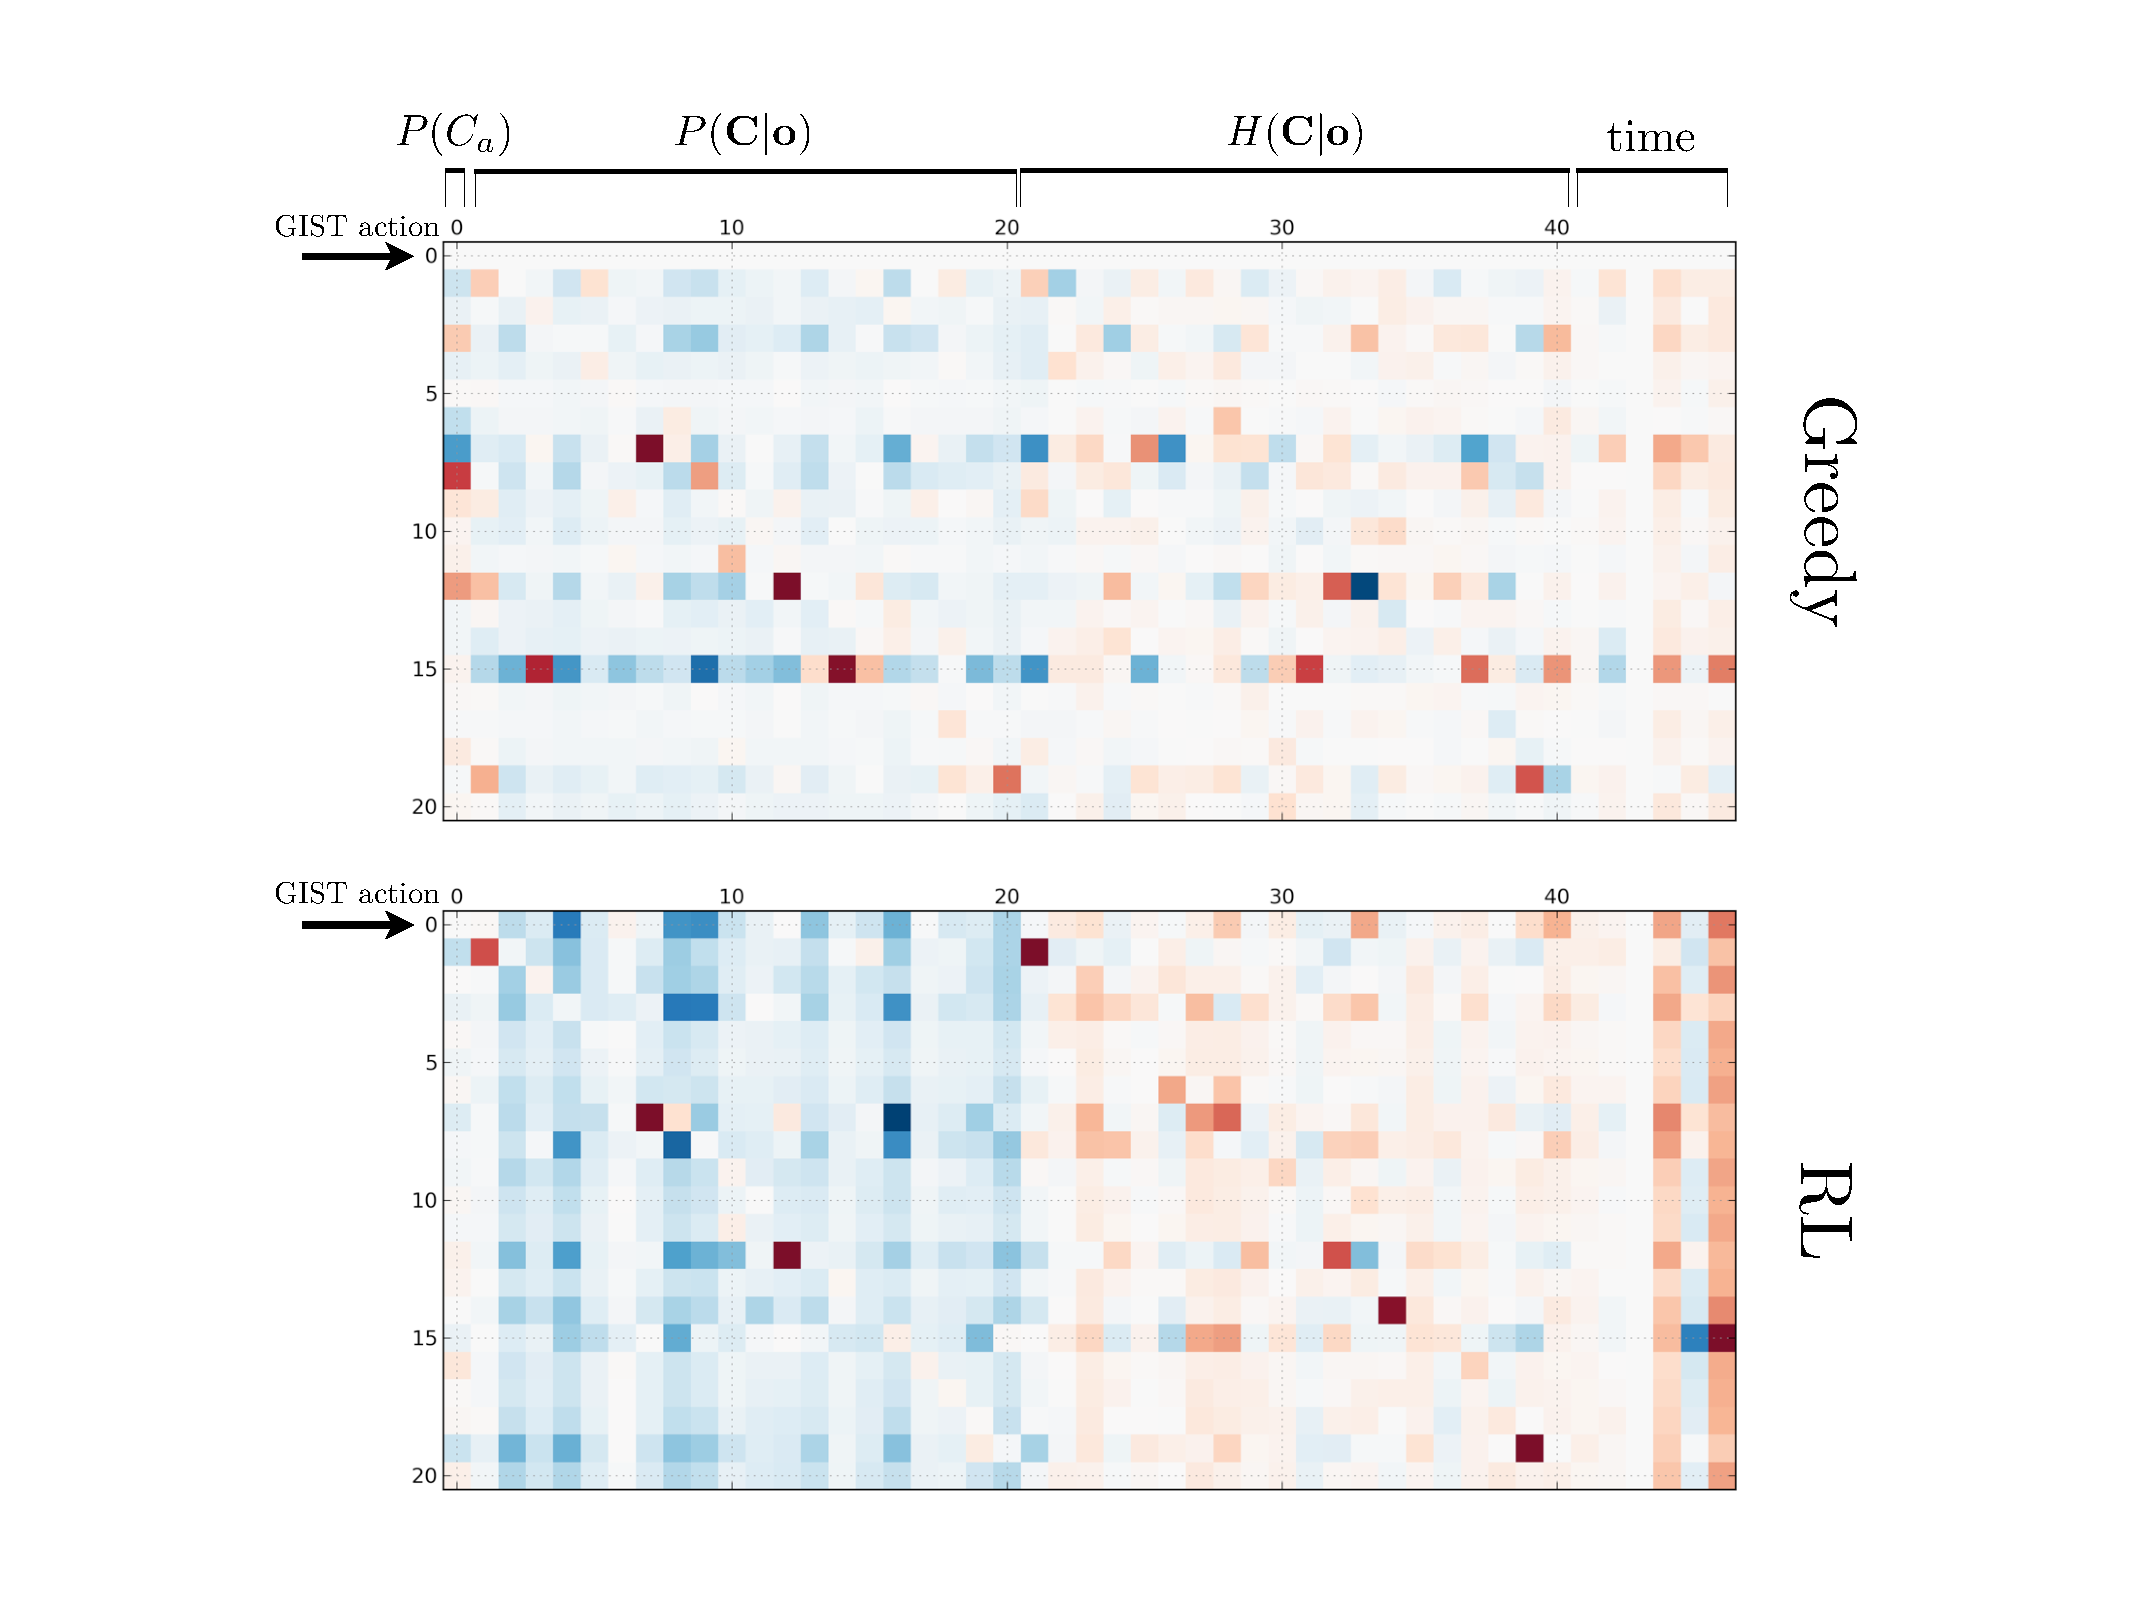
\includegraphics[width=0.87\linewidth]{../figures/weights.pdf}
\caption{
Learned policy weights $\theta_\pi$ (best viewed in color: red corresponds to positive, blue to negative values).
The first row corresponds to the scene-level action, which does not generate detections itself but only helps reduce uncertainty about the contents of the image.
Note that in the greedy learning case, this action is learned to never be taken---whereas it is shown to be useful in the reinforcement learning case.
}
\label{fig:weights}
\end{figure}

\subsection{Updating with observations} \label{sec:updating}

The bulk of our feature representation is formed by probability of individual class occurrence, conditioned on the observations so far: $P(C_0|\mathbf{o}) \ldots P(C_K|\mathbf{o})$.
This allows the action-value function to learn correlations between presence of different classes, and so the policy can look for the most probable classes given the observations.

However, higher-order co-occurrences are not well represented in this form.
Additionally, updating $P(C_i|\mathbf{o})$ presents choices regarding independence assumptions between the classes.

We evaluate two approaches for updating probabilities: \emph{direct} and \emph{MRF}.
In the \emph{direct} method, $P(C_i|\mathbf{o}) = score(C_i)$ if $\mathbf{o}$ includes the observations for class $C_i$ and $P(C_i|\mathbf{o}) = P(C_i)$ otherwise.
This means that an observation of class $i$ does not influence the estimated probability of any class but $C_i$.
$score(C_i)$ for $a_{{det}_i}$ is obtained by training a probabilistic classifier on the detections output.
$score(C_i)$ for $a_{gist}$ is obtained by training probabilistic classifiers on the GIST feature, for all classes.

The \emph{MRF} approach employs a pairwise fully-connected Markov Random Field (MRF), as shown in Figure~\ref{fig:figure1}, with the observation nodes set to $score(C_i)$ appropriately, or considered unobserved.

The graphical model structure is set as fully-connected, but some classes are overwhelmingly unlikely to co-occurr in our dataset.
Accordingly, the graph edge weights are learned with $L_1$ regularization, which obtains the desired sparse structure \cite{Lee2006}.
All parameters of the model are trained on fully-observed data, and Loopy Belief Propagation inference is implemented with an open-source graphical model package \cite{Jaimovich2010}.
% As exact inference is generally intractable in this model, we use Loopy Belief Propagation; although it does not provide general convergence guarantees, it has been shown to work well empirically on similar tasks \cite{Desai2009}.

\section{Evaluation} \label{sec:evaluation}

We use one-vs-all deformable part-model classifiers on a HOG featurization of the image \cite{Felzenszwalb2010a}, with associated linear classification of the detections.

\begin{figure}[h!]
\centering
\subfloat[Occurence of a class with another]{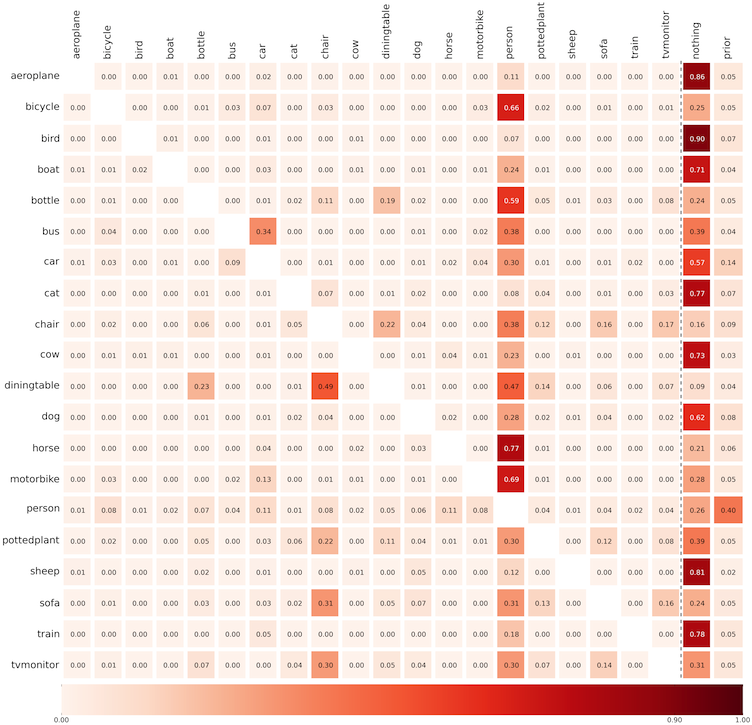
\includegraphics[]
    {../figures/full_pascal_trainval_stats/cooccur_trim.png}} \hfill
\subfloat[Occurence of a class with two others]{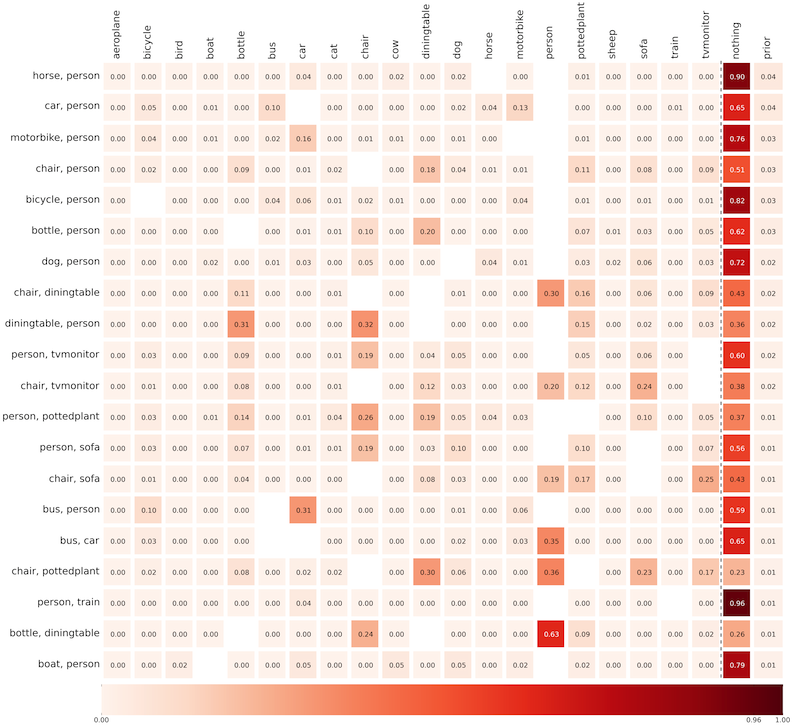
\includegraphics[]
    {../figures/full_pascal_trainval_stats/cooccur_second_order_trim.png}}
  \caption{
  Co-occurrence statistics on the training portion of the PASCAL VOC 2007 dataset.
  In the first plot, a (row,column) cell shows the probability that an image that contains an object of the row class also contains an object of the column class.
  Accordingly, in the second plot, the probability that an image containing objects of the two classes listed in the row also contains an object of the column class.
  }
  \label{fig:dataset_stats}
\end{figure}

To summarize \autoref{sec:}, we evaluate our system in the multi-class, multi-label detection regime.
We evaluate on a popular detection challenge task: the PASCAL VOC dataset \cite{pascal-voc-2010}.
As shown in \autoref{fig:dataset_stats}, the dataset exhibits a rather modest amount of class co-occurrence, which puts our model in a disadvantaged setting.
$60\%$ of the images in the training set have only one class; $30\%$ have two classes, $7\%$ have three classes, and almost none have more.

Using the 2007 version of the dataset, we train on the training and validation data and test on the test set.
We run our policies on all images in the test set, cutting off execution at $T_d$.

To evaluate performance at a given time, we gather all detections and the classification answers found to this point in all the recognition episodes.
As described before, we evaluate detection performance by averaging per-image performance in the multi-class regime.
We evaluate classification performance by pooling the ground truth across the dataset, in standard procedure.

We establish the baseline performance of our system by selecting actions randomly at each step.
The time setting for our evaluation is $T_s=0$, $T_d=20$ (in seconds).
As shown in Figure~\ref{fig:results_manual}, the random policy results in a roughly linear gain of performance vs. time.

To establish an upper bound on performance, we also plot the Oracle curve, obtained by re-ordering the actions with the hindsight of the results they produced.
Note that the curves turn downward in this setting: this is due to the different performance levels of the detectors: as the weaker detectors are inevitably run, they introduce more false positives and false negatives than true positives.

\begin{figure}[h!]
\centering
\subfloat[Detection]{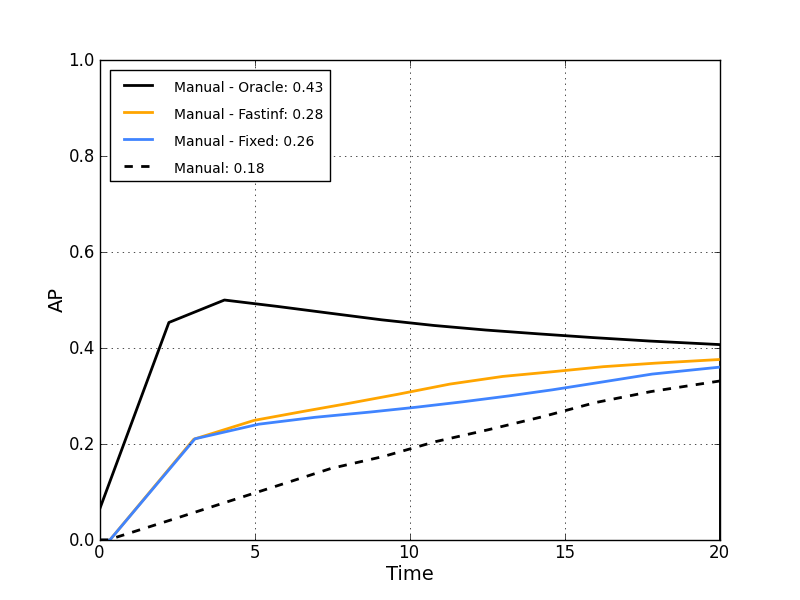
\includegraphics[width=0.78\linewidth]
    {../figures/manual_plots_det_avg.png}} \\
\subfloat[Classification]{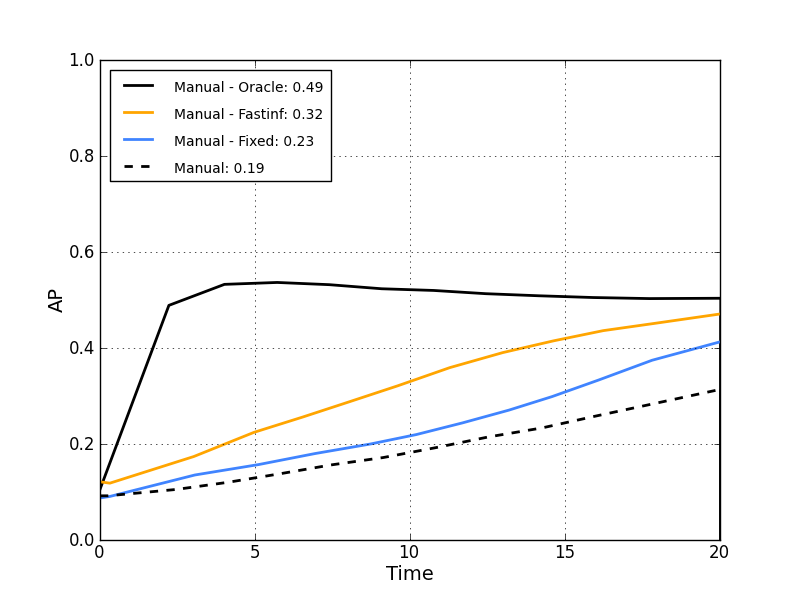
\includegraphics[width=0.78\linewidth]
    {../figures/manual_plots_cls_whole.png}}
  \caption{Heuristic value function.}
  \label{fig:results_manual}
\end{figure}

Figure~\ref{fig:results_manual} also shows the performance of our policy with the heuristic value function and two inference models: the MRF model and a simple fixed-order model that follows the priors.
We can see that due to the dataset bias, the fixed-order policy performs well at first (the person class is disproportionately likely to be in the image), but is overtaken by the proper inference model as execution goes on.

\begin{figure}[h!]
\centering
\subfloat[Detection]{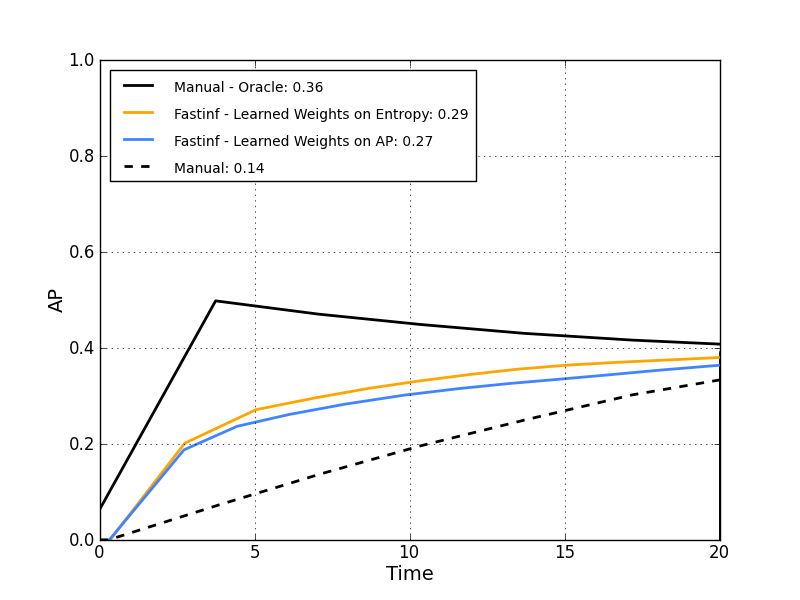
\includegraphics[width=0.78\linewidth]
    {../figures/entropy_plots_det_avg.png}} \\
\subfloat[Classification]{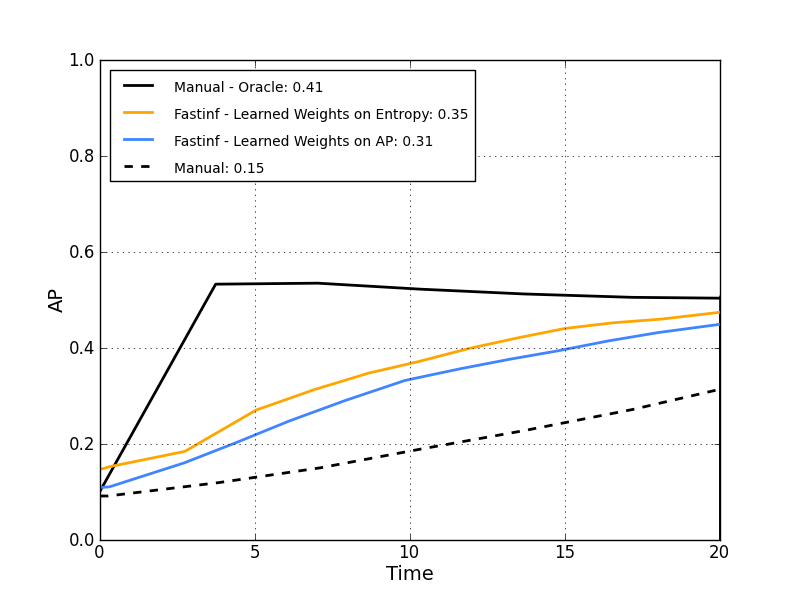
\includegraphics[width=0.78\linewidth]
    {../figures/entropy_plots_cls_whole.png}}
  \caption{Entropy reward function.}
  \label{fig:results_entropy}
\end{figure}

Figure~\ref{fig:results_entropy} shows the performance of the polices with learned weights, comparing our two reward functions.
We found the entropy-based reward to work better than the AP-based reward.

A notable difference between the MRF inference model and the fixed-order model was in the weights learned: while the fixed-order model learned weights onto the bias feature only, the MRF inference model learned weights onto a mix of the entropy and probability features.
\section{Recognition Problems and Related Work}

We deal with a dataset of images $\mathcal{D}$, where each image $\mathcal{I}$ contains zero or more objects.
Each object is labeled with exactly one category label $k \in \{1, \dots, K\}$.

The multi-class, multi-label \textbf{classification} problem asks whether $\mathcal{I}$ contains at least one object of class $k$.
We write the ground truth for an image as $\mathbf{C}=\{C_1,\dots,C_K\}$, where $C_k \in \mathbb{B} = \{0,1\}$ is set to $1$ if an object of class $k$ is present.

The \textbf{detection} problem is to output a list of bounding boxes (sub-images defined by four coordinates), each with a real-valued confidence that it encloses a single instance of an object of class $k$, for each $k$.
The answer for a single class is given by an algorithm $\emph{detect}(\mathcal{I},k)$, which outputs a list of sub-image bounding boxes $B$ and their associated confidences.

The answer is evaluated by plotting precision vs. recall across dataset $\mathcal{D}$ (by progressively lowering the confidence threshold for a positive detection).
The area under the curve yields the Average Precision (AP) metric, which has become the standard evaluation for recognition performance on challenging datasets in vision \cite{pascal-voc-2010}.
A common measure of a correct detection is the PASCAL overlap: two bounding boxes are considered to match if they have the same label and the ratio of their intersection to their union is at least $\frac{1}{2}$.

To highlight the hierarchical structure of these problems, we note that (1) the confidences for each sub-image $b \in B$ may be given by $\emph{classify}(b,k)$; (2) correct answer to the detection problem also answers the classification problem.

Multi-class performance is evaluated by averaging the individual per-class AP values.
Since our use case is motivated by a potential advertising system, we generalize this metric to a weighted average, with the weights set by the \emph{values} of the classes.

%\subsection{Related Work}
The literature on object recognition is vast.
Here we briefly summarize work that sufficiently contextualizes our contribution:

\myparagraph{Single-class detection}
The best recent performance has come from detectors that use gradient-based features to represent objects as either a collection of local patches or as object-sized windows \cite{Dalal2005,Lowe2004}.
Classifiers are then used to distinguish between featurizations of a given class and all other possible contents of an image window.
%
Window proposal is often done exhaustively over the image space, as a ``sliding window''.
Using ``jump windows'' (window hypotheses voted on by local features) as region proposals is another common idea~\cite{Vedaldi2009,Vijayanarasimhan2011}.
For local feature-based approaches, a bounded search over the space of all possible windows works reasonably well~\cite{Lampert2008a}.
%
None of the best-performing systems treat window proposal and evaluation as a closed-loop system, with feedback from evaluation to proposal.
Some work has been done on this topic, mostly inspired by ideas from biological vision and attention research~\cite{Butko2009,Vogel2008,Paletta2005}.

\myparagraph{Context}
Context has a foundational role in vision.
One source of context is the scene or other non-detector cues; the most common scene-level feature is the GIST \cite{Oliva2001a} of the image.
For the commonly used PASCAL VOC dataset \cite{pascal-voc-2010}, GIST and other sources of context are quantitatively explored in~\cite{Divvala2009}. 
%
Another source is inter-object context, shown to be useful for improving detection \cite{Torralba2004}.
A critical summary of the main approaches to using context for object and scene recognition is given in \cite{Galleguillos2010}.

\myparagraph{Multi-Class Detection}
Work on inherently multi-class detection focuses largely on making detection time sublinear in the number of classes through sharing features \cite{Torralba2007,Fan2005,Razavi2011}.
A proposed post-processing extension to detection systems uses structured prediction to incorporate multi-class context as a principled replacement for the common post-processing step of non-maximum suppression \cite{Desai2009}.

\myparagraph{Cascades}
An early success in efficient object detection used simple, fast features to build up a \emph{cascade} of classifiers, which then considered image regions in a sliding window regime \cite{Viola2001}.
Although the simple features and classifiers of this method have been surpassed by more complex detectors, the idea of cascading classifier evaluations is still often used.
Most recently, cyclic optimization has been applied to optimize cascades with respect to feature computation cost as well as classifier performance \cite{Chen2012}.
However, cascades are not dynamic policies---they cannot change the order of execution based on observations obtained during execution, which is our goal.

\myparagraph{Anytime Algorithms and Active Classification}
Anytime performance in vision systems is a surprisingly little-explored idea.
A recent application to the problem of visual detection picks features with maximum value of information in a Hough-voting framework, and explicitly evaluates performance vs. time \cite{Vijayanarasimhan2010}. 
There has also been work on active classification \cite{Gao2011} and active sensing \cite{Yu2009}, in which intermediate results are considered in order to decide on the next classification step.
This line of work is closest to our approach.
Most commonly, the scheduling in these approaches is greedy with respect to some quantity such as expected information gain.
In contrast, we are able to learn policies that take actions without any immediate reward.

\section{Future Work}
\paragraph{Extra-detection actions}
In our implementation of the system, we leave open the possibility of extra-detection actions---those actions that may modify the belief state but not generate any detections directly.
In fact, we implemented one such action: a regression from the GIST \cite{Oliva2001a} feature of the image to object class presence.
In our experiments, this action was always taken first in every policy evaluation; we did not observe an improvement over not using this special action, but leave the question open for further investigation.

\paragraph{Policy Iteration}
While our current implementation shows significant gains over baseline, the gap between our policies' performance and the oracle performance shows that there is yet room to improve.
In particular, we are looking at using the general method of policy iteration to derive approximations of the value function that are able to capture not just greedy but expected rewards to the end of the episode.
Solving POMDPs, of which our stated problem is an example, has not in general been robustly done for problems of this size \cite{Murphy2000,Ng2000}, but there are promising relaxes approaches \cite{Kwok2004}.



\bibliographystyle{splncs}
\bibliography{sergeyk-bibtex,misc}

\end{document}
